\section{Motivation}

Since the advent of modern digital communications in the 20th century there has been an explosion in the demand for wireless spectrum.  As a result spectrum is becoming an increasingly scare resource\cite{scarcity}.  This demand is a direct result of the availability and relatively inexpensive cost of such wireless device.  Therefore in such envirorments as militaristic theatres the probability of interfering transmissions, intended and unintended, has steadily grown to a point where techniques need to be consider to combat such occurrences.  More directly, in such situations when interfering signals are partially or completely understood measures can be taken to overcome such difficulties.\\

In military theatres it is extremely common to observe friendly operated high-power broadband jamming signals\cite{frater}.  Such devices exists as part of group convoys in several branches of the military and in many other forms in contested territories or war-zones.  Unfortunately such devices block both friendly and hostile communications, and current anti-jamming techniques haven't provided a viable solution to this problem.  Therefore new avenues should be considered, utilizing more flexible radio technologies.\\

Understanding how to overcome such challenges is a complex task; with vastly different transmission envirorments and differing operating devices and operating standards.  A new system that could combat such downfalls should rely on all friendly information, or be able to construct solutions of its own from a set of tools given to the radio.  Such tools should be flexible and easily modified, changed, or improved.  This ability to easily change or adapt is a key feature as the technical requirements can change from day to day, or between branches of the military itself. As such a solution should have the following attributes:

\begin{itemize}
\item \textbf{Flexible:}

\item \textbf{Resilient:}

\item \textbf{Hardened:} in changing enviroments

\end{itemize}


\section{State of the Art}

Current implementations in anti-jamming technology lies on the strateling point of hardware and software in the communications world.  This is true because hardware provides the speed and performance needed for digital data transmission, while software provides higher level intelligence and flexibility in such layers as the media access control layer and the network layer of the Open Systems Interconnect (OSI) model\cite{Zimmermann}.  For anti-jamming applications, high intelligence allows for mobility again the jammer.  Therefore a large implementation in software must be considered when investigating anti-jamming technics.\\

\begin{figure}
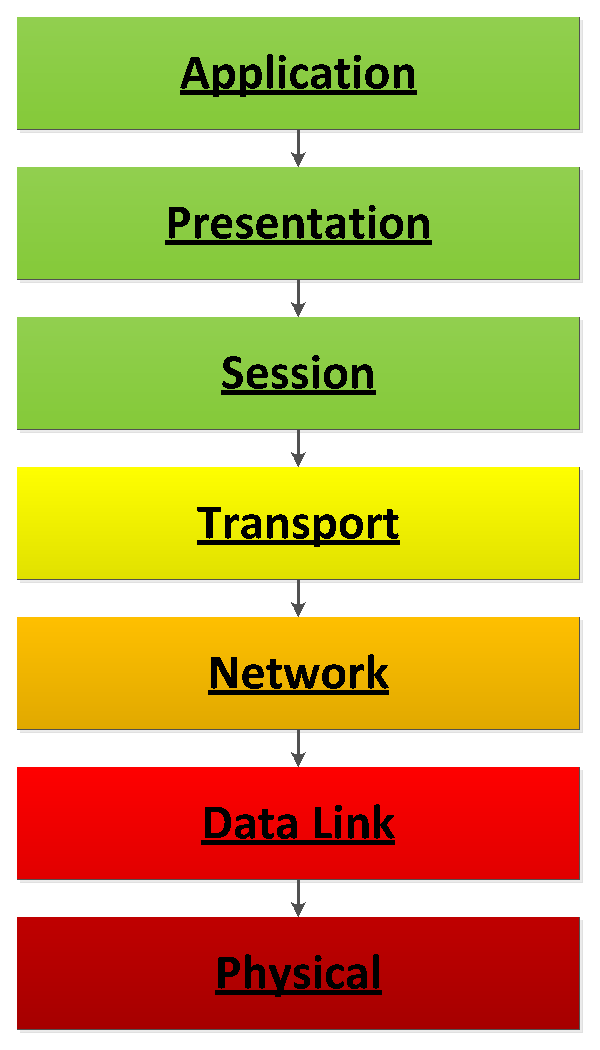
\includegraphics[scale=0.10]{OSI_model.eps}
\end{figure}

Current anti-jamming technics include channel hopping, spatial retreat, jammed area mapping, node escape, retreat restoration, frame masking, and many more\cite{1}.  All of these techniques use mechanisms of evasion or despection.  These can be quite effective when attacked by generally narrowband, non-dynamic/non-learning jammers.  In the case of wide and ultra-wide band jammers, they fail miserably.  This wide-band enviorment is the primary situation of interest, and it generally considered a hopeless scenario.  These anti-jam technics are design for specific situations and jammers.\\

Let us first examine these anti-jamming technics which are broken down into three primary categories: Proactive countermeasures, Reactive countermeasures, and Mobile agent-base countermeasures\cite{1}.  Reactive countermeasures relies on a varying array of detection mechanisms first to determine if that node is being jammed.  These detection methods  must be coupled with a countermeasure or the scheme is in operable.  Examples of these detection methods include a transmitter-based approach and a receiver-based detection.  In a transmitter-based approach, such as ad-hoc networks, a decision algorithm is used based on four metrics: Packet Delivery Ratio (PDR), Received Signal Strength Indicator (RSSI), Physical rate, and Noise levels\cite{3}.  In the receiver-based detection additional information must be injected into frames to help the receiver determine the number of frames lost.  Since frames can be easily lost in wireless transmissions, the receiver is handicapped when determining the number of retransmissions that have occurred.  In the transmitter the PDR is deterministicly determined by the data-link layer, sequence numbers must be added to frames for the receiver to accurately calculate the PDR\cite{3}.  Several other detection methods exist including using a detected detector, cooperative detection among nodes in a wireless network, and more sophisticated methods of RF fingerprinting\cite{3}.\\

Once the jammer has been detected the reactive countermeasures come into play.  Many evasion techniques exists to combat narrowband jammers such as: channel hoping, spatial retreat, retreat restoration, hybrid attacks, and many cognitive radio approaches\cite{2}.  Many of these technics utilize the network itself to adapt to the jammer, which is an appropriate assumpt because without a network communications are irrelivant.  Channel hopping is quite simple and can be considered easiet to implement.  If a channel is begining jammed simply ``hop'' to another channel.  This is easily defeated in two cases, the first the jammer follows you or the jammer is simply wideband capable.  The second, spatial retreat, is a mechanism to physically evade the areas being jammed. Based on the detection algorithm all nodes in a network try to estimate the jammed region and flee physically in the direction of safer place. Based on their estimation about the jammed region, nodes will utilize shortest path algorithms to determine location of retreat\cite{5}.  Retreat restoration is focused around how to rebuild a network once the jammer has left.  Retreat restoration can be done by coordinated or uncoordinated communication, and the transmissions are based on a pre planned hop patterns among nodes\cite{6}.\\

There also exists systems that are design to resist jamming proactively.  These hybrid systems\cite{7} utilize preventatives measure to resist jamming such as frequency hopping spread spectrum (FHSS).  Spread-spectrum signals are highly resistant to narrowband jamming, unless the jammer has knowledge of the spreading key. In military applications the spreading key is generally created using a crytographic function\cite{sterling}.  More hybrid solutions include synchronous and asynchronous spectral multiplexing where intermediary nodes are used to communicate at multiple channels.  When a node changes its channel because of jamming a neighbor will heal that connection by communicating  with the node on its new channel and rest of the network on the old channel\cite{8}.


The largest problem with these techniques is they all have are designed to combat narrowband jammers, and even friendly jammers.  If high powered wideband jammers enter the equation, all of these solutions fall apart.  Note these techniques primarily exploit the dimensionality of their envirmonent by simply avoiding the jammer, and all techniques require intelligent flexible hardware solutions.   To implement such solutions requires suffisticated hardware implementations, that can be quite rigid for rapidly changing communication envirorments and adversaries.  To compensate solutions that push more of the radio operations from their original rigid hardware implementations into the more flexible software domain, provide a more cost effective and elligent solution.  These software focused radios, also know as Software defined radios, have provided a solid platform for very adaptive anti-jamming technologies under the name cogntive radios.  These radios have the ability to easily learn and adapt to their envirorment, which is the primary requirement of anti-jamming devices.\\

As mentioned above, it is quite common for the military to self-jam its own channels.  Unfortunately this can hinder their own use unintenially.  These disrupted users are known as ``disadvantage users''.  They are commonly small mobile hand held devices and cannot simply overcome the jammer computationally or in raw power; therefore, more manageable and eligent solutions must be considered for such disadvantaged users.  Beside self-jammming, adversarial jammers must also be considered.  Fortunately certain characteristics can be statistically exploited if these jammer abide by certain properties. Since adversarial jammers tend to inject random data or energy to block communication, if these transmissions can be shown to repeat they can be exploited.  In the case of self-jamming, the signal characteristic can be know \textit{a priori}; therefore they also can exploted or removed, negating the effects of such devices.  Such scheme must consider the energy or symbols of the jammmer that are orthoganol and/or non-orthoganol to the symbols of the communication itself.\\


The goal of this project is to exploit a self-jammed and statiscially determistic adversarially jammed channel, throught the utilization of cognitive radio, implemented on a software defined radio platform.  Software defined radios, defined as the intersection between hardware radios and computer software\cite{4}, provide a platform flexible enough to support highly intelligence operations such that anti-jamming requires.  A proposed adaptive signal processing software solution for mitigating the effects of both intentional and unintentional jamming (including wideband jamming) via the combination of antenna subset selection, spectral subtraction, and blind source separation (BSS) techniques in order to extract specific transmissions from a mixture of intercepted wireless signals. The goal of our proposed solution, called BLInd Spectrum Separation (BLISS), is to enable reliable, high throughput, and robust end-to-end wireless communications.\\

This work is a continuation of the work done through a collaberation of the United States Naval Academy, Worcester Polytechnic Insitute, and other external contractors.  Primarily literature surveys and early simulations were completed or attempted before the transition of the project to the work done by this thesis.  Credit is given to the following authors and there coensiding section or block as follows: Srikanth Pagadarai and Ryan Dobins Blind Source Separation, Robert Over Spectral Subtraction, Robert Capizzio Benjamin Hilbern and Dr. Christopher Anderson Antenna Subset Selection.  This document examines the provided work dones by these individuals in detail, except for the topics in Antenna Subset Selection due to time constraints.\\

\section{Thesis Contributions}

This thesis will contribute the following to the wireless communications and signal processing research communities:

\begin{itemize}
\item A basis for blind source separation of define subset of signals, and tools on estimating and removing those signals.

\item A practical implementation using over the air communications of a anti-jamming sytem utilizing software defined radios. This implementation will tackle wideband non-orthoganol and orthoganol jamming, and provide evidence of probability of operational.
\end{itemize}


\section{Thesis Organization}

This thesis will be organized into the following chapters.  Chapter 2 provides the necessary background to understand basic communication system design, anti-jamming technics, and signal processing.  Chapter 3 puts forward a theoritical simulations and a design of a physical anti-jamming system.  Chapter 4 presents the results of the physical implement and analysis of its findings.  Chapter 5 concludes the thesis, summarizing the accomplishments and outlines possible future work.
